\chapter{Antiderivatives}

In your study of calculus, you have learned about derivatives, which
allow us to find the rate of change of a function at any given
point. Derivatives are powerful tools that help us analyze the
behavior of functions. Now, we will explore another concept called
antiderivatives, which are closely related to derivatives.\index{Antiderivatives}

An antiderivative, also known as an integral or primitive, is the
reverse process of differentiation. It involves finding a function
whose derivative is equal to a given function. In simple terms, if you
have a function and you want to find another function that, when
differentiated, gives you the original function back, you are looking
for its antiderivative.

The symbol used to represent an antiderivative is $\int$. It is called
the integral sign. For example, if $f(x)$ is a function, then the
antiderivative of $f(x)$ with respect to $x$ is denoted as $\int f(x)
, dx$. The $dx$ at the end indicates that we are integrating with
respect to $x$.

Another way to state this is that $F$ is the antiderivative of $f$ on 
an interval, $I$, if $F'(x) = f(x)$ over the interval. The 
relationship between $f$ and $F$ is discussed more in the chapter on 
the Fundamental Theorem of Calculus. 

Finding antiderivatives requires using specific techniques and
rules. Some common antiderivative rules include:

\begin{itemize}
\item The power rule: If $f(x) = x^n$, where $n$ is any real number
  except $-1$, then the antiderivative of $f(x)$ is given by $\int
  f(x) , dx = \frac{1}{n+1}x^{n+1} + C$, where $C$ is the constant of
  integration.

\item The constant rule: The antiderivative of a constant function is
  equal to the constant times $x$. For example, if $f(x) = 5$, then
  $\int f(x)\, dx = 5x + C$.

\item The sum and difference rule: If $f(x)$ and $g(x)$ are functions,
  then $\int (f(x) + g(x)) \, dx = \int f(x) \, dx + \int g(x) \,
  dx$. Similarly, $\int (f(x) - g(x)) , dx = \int f(x) \, dx - \int
  g(x) \, dx$.
\end{itemize}

Antiderivatives have various applications in mathematics and
science. They allow us to calculate the total accumulation of a
quantity over a given interval, compute areas under curves, and solve
differential equations, among other things.

\section{General Antiderivatives}

It is important to note that an antiderivative is not a unique
function. Since the derivative of a constant is zero, any constant
added to an antiderivative will still be an antiderivative of the
original function. This is why we include the constant of integration,
denoted by $C$, in the antiderivative expression.

Stated formally, if $F$ is an antiderivative of $f$ on interval $I$, 
then the most general antiderivative of $f$ on $I$ is $F(x) + C$, 
where $C$ is an arbitrary constant. 


A concrete example of this is $f(x) = x^2$. Let us define $F(x)$ such 
that $F'(x) = f(x)$. That is, there is some function $F$ such that the 
derivative of $F$ is $x^2$. One possible solution for $F$ is $F(x) = 
\frac{1}{3} x^3$. You can check using the power rule that $\frac{d}{dx} 
F(x) = f(x)$. What if we added or subtracted a constant from $F$? Let 
us define $G(x) = \frac{1}{3} x^3 + 2$. Well, $G'(x) = f(x)$ also! 
Same for $H(x) = \frac{1}{3} x^3 - 7$. Several possible antiderivatives 
of $f(x) = x^2$ are shown in figure \ref{fig:antideriv}. 

\begin{figure}
	\centering
	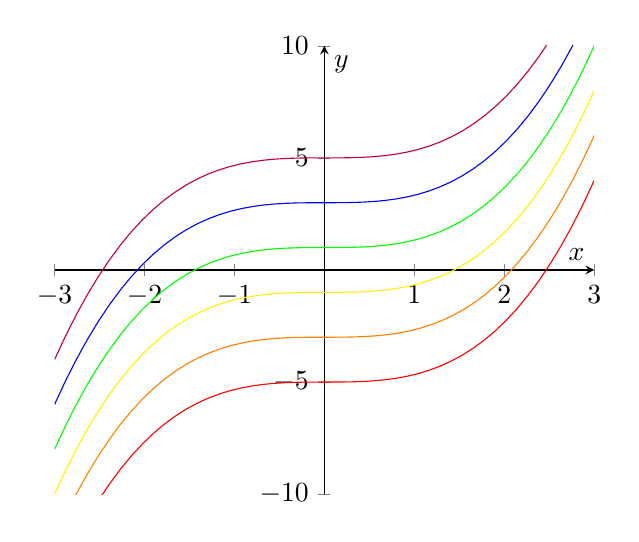
\begin{tikzpicture}
		\begin{axis}
			[axis lines = center, 
			xmin=-3, xmax=3, xlabel=$x$, 
			ylabel=$y$, ymin=-10, ymax=10]
		\addplot[red, samples=50, domain=-3:3]{(1/3)*x^3 - 5};
		\addplot[orange, samples=50, domain=-3:3]{(1/3)*x^3 - 3};
		\addplot[yellow, samples=50, domain=-3:3]{(1/3)*x^3 - 1};
		\addplot[green, samples=50, domain=-3:3]{(1/3)*x^3 + 1};
		\addplot[blue, samples=50, domain=-3:3]{(1/3)*x^3 +3};
		\addplot[purple, samples=50, domain=-3:3]{(1/3)*x^3 + 5};
		\end{axis}
	\end{tikzpicture}
	\caption{Several possible solutions to $F'(x) = x^2$}
	\label{fig:antideriv}
\end{figure} 

Since taking a derivative "erases" any constant, you must always add 
back in the unknown constant, $C$, when finding the general 
antiderivative. 

\section{Specific Antiderivatives}
If you are given a condition, you can often solve for $C$ and find a 
specific antiderivative. For example, suppose that in addition to 
knowing that $F'(x) = x^2$, we also know that $F(3) = 2$. We can use 
the fact that $F$ passes through $(3, 2)$ to find the value of $C$:

$$F(x) = \frac{1}{3} x^3 + C$$
$$F(3) = \frac{1}{3} (3)^2 + C = 2$$
$$39 + C = 2$$
$$C = -7$$

Therefore, the specific solution to $F'(x) = x^2$ with the condition 
that $F(3) =2$ is $F(x) = \frac{1}{3} x^3 - 7$. 

\section{Antiderivatives of Trig Functions}
We already know that $\frac{d}{dx} \sin{x} = \cos{x}$. Taking $\sin{x}$ 
to be $F(x)$ and $\cos{x}$ to be $f(x)$, we see that $F'(x) = f(x)$ 
and therefore $\sin{x}$ is the antiderivative of $\cos{x}$. 

\begin{Exercise}[label=triganti]
What is the antiderivative of $\sin{x}$? Explain your answer. 
\end{Exercise}

\begin{Answer}[ref=triganti]
Since we are finding the antiderivative of $\sin{x}$, we will define 
$f(x) = \sin{x}$. We are looking for a $F$ such that $F'(x) = \sin{x}$. 
The derivative of $\cos{x}$ is $-\sin{x} \neq f(x)$. But the derivative 
of $-\cos{x} = \sin{x} = f(x)$. Since $\frac{d}{dx} [-\cos{x}] = 
\sin{x}$, the antiderivative of $\sin{x}$ is $-\cos{x}$. 
\end{Answer}

You should have found that the antiderivative of $\sin{x}$ is 
$-\cos{x}$. Other general antiderivatives of trigonometric functions 
are presented in the table below. 

\begin{tabular}{c|c}
Function & Antiderivative\\
$\cos{x}$ & $\sin{x} + C$\\
$\sin{x}$ & $-\cos{x} + C$\\
$\sec^2{x}$ & $\tan{x} + C$\\
$\sec{x} \tan{x}$ & $\sec{x} + C$\\
$-\csc^2{x}$ & $\cot{x} + C$\\
$-\csc{x} \cot{x}$ & $\csc{x} + C$\\
\end{tabular}

Notice this is the flipped version of the derivatives of trigonometric 
functions presented in the Trigonometric Functions chapter. This hints 
at the relationship between derivatives and integrals: they are 
opposite processes. 

\section{Other Important Antidervatives}

The Power Rule only applies when $n\neq-1$. Then what is the 
antiderivative of $f(x) = \frac{1}{x}$? Recall from the chapters on 
derivatives that $\frac{d}{dx} \ln{x} = \frac{1}{x}$. Therefore, the 
general antiderivative of $\frac{1}{x}$ is $\ln{|x|} + C$. We have to 
take the absolute value because of the domain restrictions of $\ln{x}$. 

Since the derivative of $e^{x}$ is $e^{x}$, it follows that the general 
antiderivative of $e^{x}$ is $e^{x} + C$. What if there is a 
multiplying factor in the exponent, such as $e^{kx}$? Recall that 
$\frac{d}{dx} e^{kx} = k e^{kx}$. It follows that $\frac{d}{dx} 
\frac{1}{k} e^{kx} = e^{kx}$. Therefore, the general antiderivative of 
$e^{kx}$ is $\frac{1}{k} e^{kx} + C$. 

Often, the base of an exponential function isn't $e$. We can also find 
the general antiderivative of $b^{x}$, where $b \neq e$. Recall that 
$\frac{d}{dx} b^x = \ln{b} b^x$. Therefore $\frac{d}{dx} \frac{1}{\ln{b}} 
b^x = b^x$, and the general antiderivative of $b^x$ is $\frac{b^x}{\ln{b}}$. 

\section{Higher order antiderivatives}
What if we are given the second order derivative, or a higher order? 
Take this example: $f''(x) = 2x+3e^x$. The antiderivative of $f''$ is 
$f'$. Applying the Power Rule and knowing the antiderivative of $e^x$ 
is $e^x$, we find that $f'(x) = x^2 + 3e^x + C_1$. We designate the 
constant as $C_1$ because we'll have to determine the antiderivative a 
second time and we don't want to confuse our constants with each other.
 To find $f$, we apply the Power Rule again, and we find that $f(x) = 
\frac{1}{3} x^3 + 3e^x + C_1x + C_2$. You can check if this is correct 
by taking the derivative of $f(x)$ twice, which should yield the 
$f''(x)$ originally given. 

In summary, antiderivatives are the reverse process of
differentiation. They help us find functions whose derivatives match a
given function. Understanding antiderivatives is crucial for various
advanced calculus concepts and real-world applications.

Now, let's explore different techniques and methods for finding
antiderivatives and discover how they can be applied in solving
problems.

\section{Additional Practice}

\begin{Exercise}[label=antideriv1]
	A particle moving in a straight line has an acceleration given by 
	$a(t) = 6t + 4$. If its initial velocity is $-6 \frac{cm}{s}$ and 
	its initial position is $9 cm$, what is the function $s(t)$ that 
	describes the particle's position?
\end{Exercise}

\begin{Answer}[ref=antideriv1]
	First, we will find $v(t)$ by taking the antiderivative of $a(t)$ and 
	using the initial condition $v(0) = -6$
	$$\int 6t + 4 \ , dt = 3t^2 + 4t + C = v(t)$$
	$$v(0) = 3(0)^2 + 4(0) + C = -6$$
	$$C = -6$$
	Therefore, the velocity function is $v(t) = 3t^2 + 4t - 6$. Now we 
	repeat the process to find $s(t)$:
	$$\int 3t^2 + 4t - 6 \ , dt = t^3 + 2t^2 - 6t + C = s(t)$$
	$$s(0) = (0)^3 + 2(0)^2 - 6(0) + C = 9$$
	$$C = 9$$
	Therefore, the position function is $s(t) = t^3 + 2t^2 - 6t + 9$. 
\end{Answer}

\begin{Exercise}[label=antideriv2]
	Let $f'(x) = 2\sin{x}$. If $f(\pi) = 1$, write an expression for 
	$f(x)$. 
\end{Exercise}

\begin{Answer}[ref=antideriv2]
	The antiderivative of $\sin{x}$ is $-\cos{x}$ and therefore the 
	general solution is $f(x) = -2\cos{x} + C$. We use the given 
	condition, $f(\pi) = 1$ to find $C$:
	$$f(\pi) = -2\cos{\pi} + C = 1$$
	$$C = 1 + 2\cos{\pi} = 1 + 2(-1) = -1$$
	Therefore, the specific solution is $f(x) = -2\cos{x} - 1$
\end{Answer}

\begin{Exercise}[label=antideriv3]
	Find the general antiderivatives of the following functions:
	\begin{enumerate}
	\item $f(x) = x^2 + 2x - 4$
	\item $g(x) = \sqrt[3]{x^2} + x\sqrt{x}$
	\item $h(x) = \frac{1}{5} - \frac{2}{x}$
	\item $r(\theta) = 2\sin{\theta} - \sec^2{\theta}$
	\end{enumerate} 	
\end{Exercise}

\begin{Answer}[ref=antideriv3]
	\begin{enumerate}
	\item By the power rule, the antiderivative of $x^2$ is 
	$\frac{1}{3}x^3$, the antiderivative of $2x$ is $x_2$, and the 
	antiderivative of $4$ is $4x$. So the general antiderivative of $f(x)$ 
	is $\frac{1}{3}x^3 + x^2 - 4x + C$
	\item We can rewrite $g(x)$ to more clearly see the powers of $x$. 
	$g(x) = x^{\frac{2}{3}} + x^{\frac{3}{2}}$. Applying the Power rule, 
	we find the general antiderivative of $g(x)$ is 
	$\frac{3}{5}x^{\frac{5}{3}} + \frac{2}{5}x^{\frac{5}{2}} + C$. 
	\item Recalling that the antiderivative of $\frac{1}{x}$ is 
	$\ln{|x|}$, the general antiderivative of $h(x)$ is $\frac{1}{5}x - 
	2\ln{|x|} + C$
	\item The antiderivative of $\sin{\theta}$ is $-\cos{\theta}$ and the 
	antiderivative of $\sec^2{\theta}$ is $\tan{x}$. Therefore, the 
	general antiderivative of $r(\theta)$ is $-2\cos{\theta} - 
	\tan{\theta} + C$
	\end{enumerate}
\end{Answer}

\begin{Exercise}[label=antideriv4]
	Find the $f$ that satisfies the given conditions:
	\begin{enumerate}
	\item $f'(\theta) = \sin{\theta} + \cos{\theta}$, $f(\pi) = 2$
	\item $f''(x) = 12x^2 + 6x - 4$, $f(0) = 4$ and $f(1) = 1$
	\end{enumerate}
\end{Exercise}
	
\begin{Answer}[ref=antideriv4]
	\begin{enumerate}
	\item The antiderivative of $\sin{\theta}$ is $-\cos{\theta}$ and the 
	antiderivative of $\cos{\theta}$ is $\sin{\theta}$. The general form 
	of $f$ is $f(\theta) = -\cos{\theta} + \sin{\theta} + C$. 
	Substituting $\theta = \pi$, we find that $f(\pi) = -\cos{\pi} + 
	\sin{\pi} + C = 1 + 0 + C = 2$, which implies $C = 1$. Therefore 
	$f(\theta) = -\cos{\theta} + \sin{\theta} + 1$.
	\item The general antiderivative of $f''$ is $f'(x) = 4x^3 + 3x^2 - 
	4x + C_1$. We don't have a condition for $f'$, so we continue to find 
	$f$. The antiderivative of $f'$ is $f(x) = x^4 + x^3 - 2x^2 + C_1x + 
	C_2$. We can find $C_2$ with the condition $f(0) = 4$. $f(0) = C_2 
	= 4$, so we know $f(x) = x^4 + x^3 - 2x^2 + C_1x + 4$. Using the 
	condition $f(1) = 1$, we find that $C_1 = 3$. Therefore, the specific 
	solution is $f(x) = x^4 + x^3 - 2x^2 + 3x - 4$. 
	\end{enumerate}
	 
\end{Answer}



